\chapter{Radio e Reti Wireless}

\section{Trasmissioni Radio}
Le trasmissioni radio sono soggette a problemi di sicurezza informatica.
Molto integrate nei sistemi:
\begin{itemize}
    \item Cancelli automatici
    \item Telecomandi automobili
    \item RFID (contactless)
    \item Wi-Fi (IEEE 802.11)
    \item Bluetooth / Zigbee / Domotica
\end{itemize}
\subsection{Basi teoriche Radio}
Nelle comunicazioni radio vengono definiti:
\begin{itemize}
    \item Trasmettitore - \textbf{TX}: colui che trasmette le informazioni;
    \item Ricevitore - \textbf{RX}: colui che riceve le informazioni;
    \item Transceiver: è un dispositivo in grado di effettuare entrambe le operazioni.
\end{itemize}

La trasmissione radio avviene eccitando un antenna, il campo elettrico viene "spostato" nell'ambiente circostante. Sostanzialmente gli elettroni in cui è immersa l'antenna (l'etere) vengono spostati dall'energia a cui la sottoponiamo.
Per poter inviare il giusto segnale ogni tipo di antenna ha la sua peculiarità e deve essere dimensionata correttamente per la trasmissione che vogliamo effettuare.
Nella ricezione invece l'antenna riceve lo "spostamento" del campo elettrico e lo invia alle componenti elettroniche a cui è collegata, i quali si occuperanno di elaborare le informazioni ricevute.\\
Per trasmettere l'antenna deve "vibrare". Questa vibrazione deve essere effettuata a una determinata frequenza, la frequenza si fa vibrare l'antenna prende il nome di "portante".
In ricezione invece un'antenna più grande risulterà e più informazioni riuscirà a ricevere (più frequenze catturate), la ricevente catturerà molte più informazioni di quelle di cui necessitiamo per questo sarà necessario filtrarle, questo processo prende il nome di sintonizzazione. La sintonizzazione non è sicurezza.

\subsection{Modulazione}
Per permettere una trasmissione dati sicura bisognerà stipulare un protocollo di comunicazione (layer 1), che prevederà come le informazioni (bit) vengono codificate e inviate dall'antenna.Esistono tre principali classi di modulazione:
\begin{itemize}
    \item Modulazione in Ampiezza (AM)
    \item Modulazione in Frequenza (FM)
    \item Modulazione in Fase (PM)
\end{itemize}
La modulazione più semplice che vedremo è l'\textbf{OOK} (on off keyring), facente parte della modulazione AM.
Il concetto alla base è trasmettere i dati accendendo (bit 1) e spegnendo (bit 0) la portante.
\begin{figure}[h!]
    \centering
    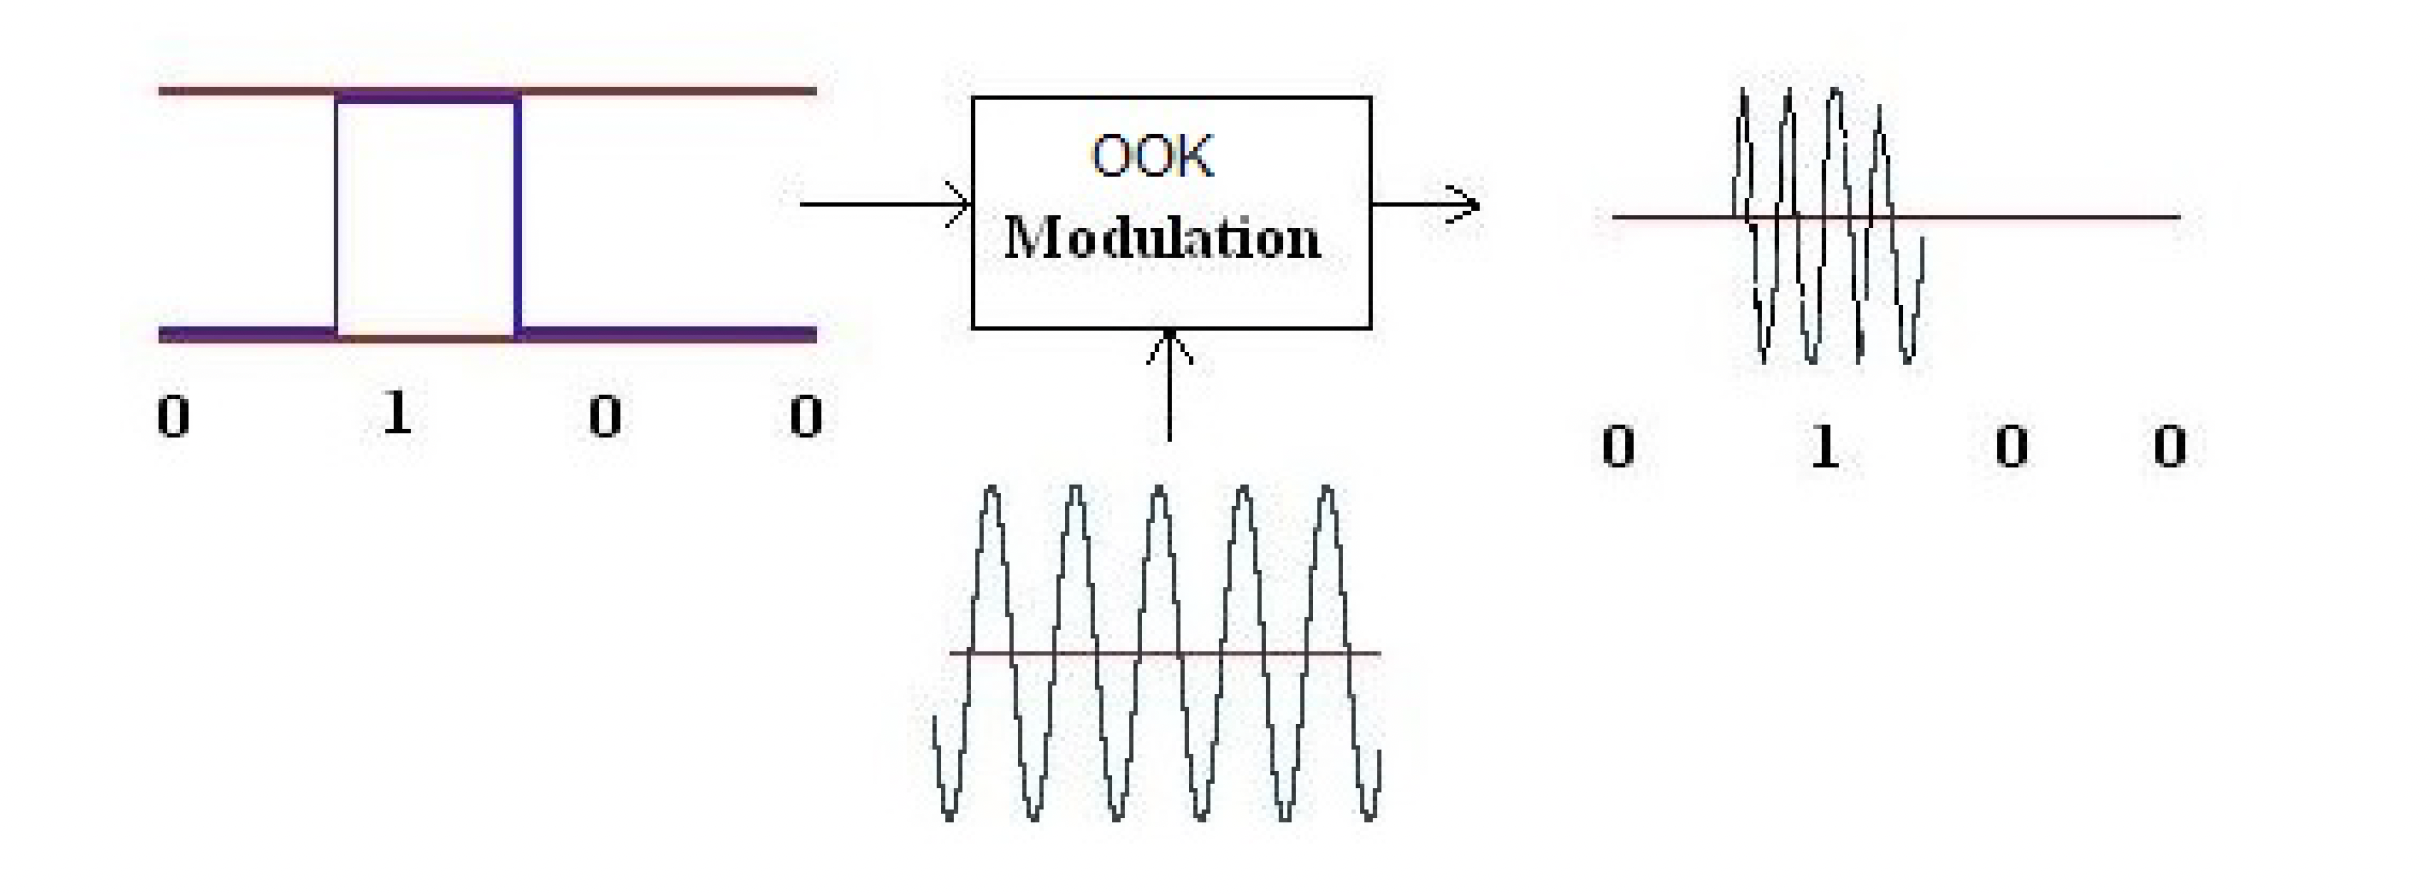
\includegraphics[width=.8\linewidth]{res/OOK.png}
    \caption{}
\end{figure}
\subsection{Jamming}
Un problema di questa modulazione è facilmente intuibile, in quanto accendendo sempre la portante non si avrà più l'invio dell'informazione, problema presente anche in altri protocolli (I2C).
Un attacco che si può effettuare con questi protocolli è mediante l'utilizzo di un \textbf{jammer}, l'idea per renderlo meno efficacie è quella di utilizzare più frequenze portanti aumentando la banda (banda larga) in questo modo il jammer dovrà utilizzare più energia per offuscarle tutte.
Un meccanismo per ovviare all'attacco tramite jammer è l'utilizzo del \.textbf{FHSS} (Frequency Hopping Spread Spectrum) che consiste nel utilizzare più portanti, con un ordine scelto a priori, per inviare le informazioni, così in caso di jamming o collisione di segnali si avrà una perdita di informazioni limitata ad una sola portate perdendo meno informazioni.
\begin{figure}[h!]
    \centering
    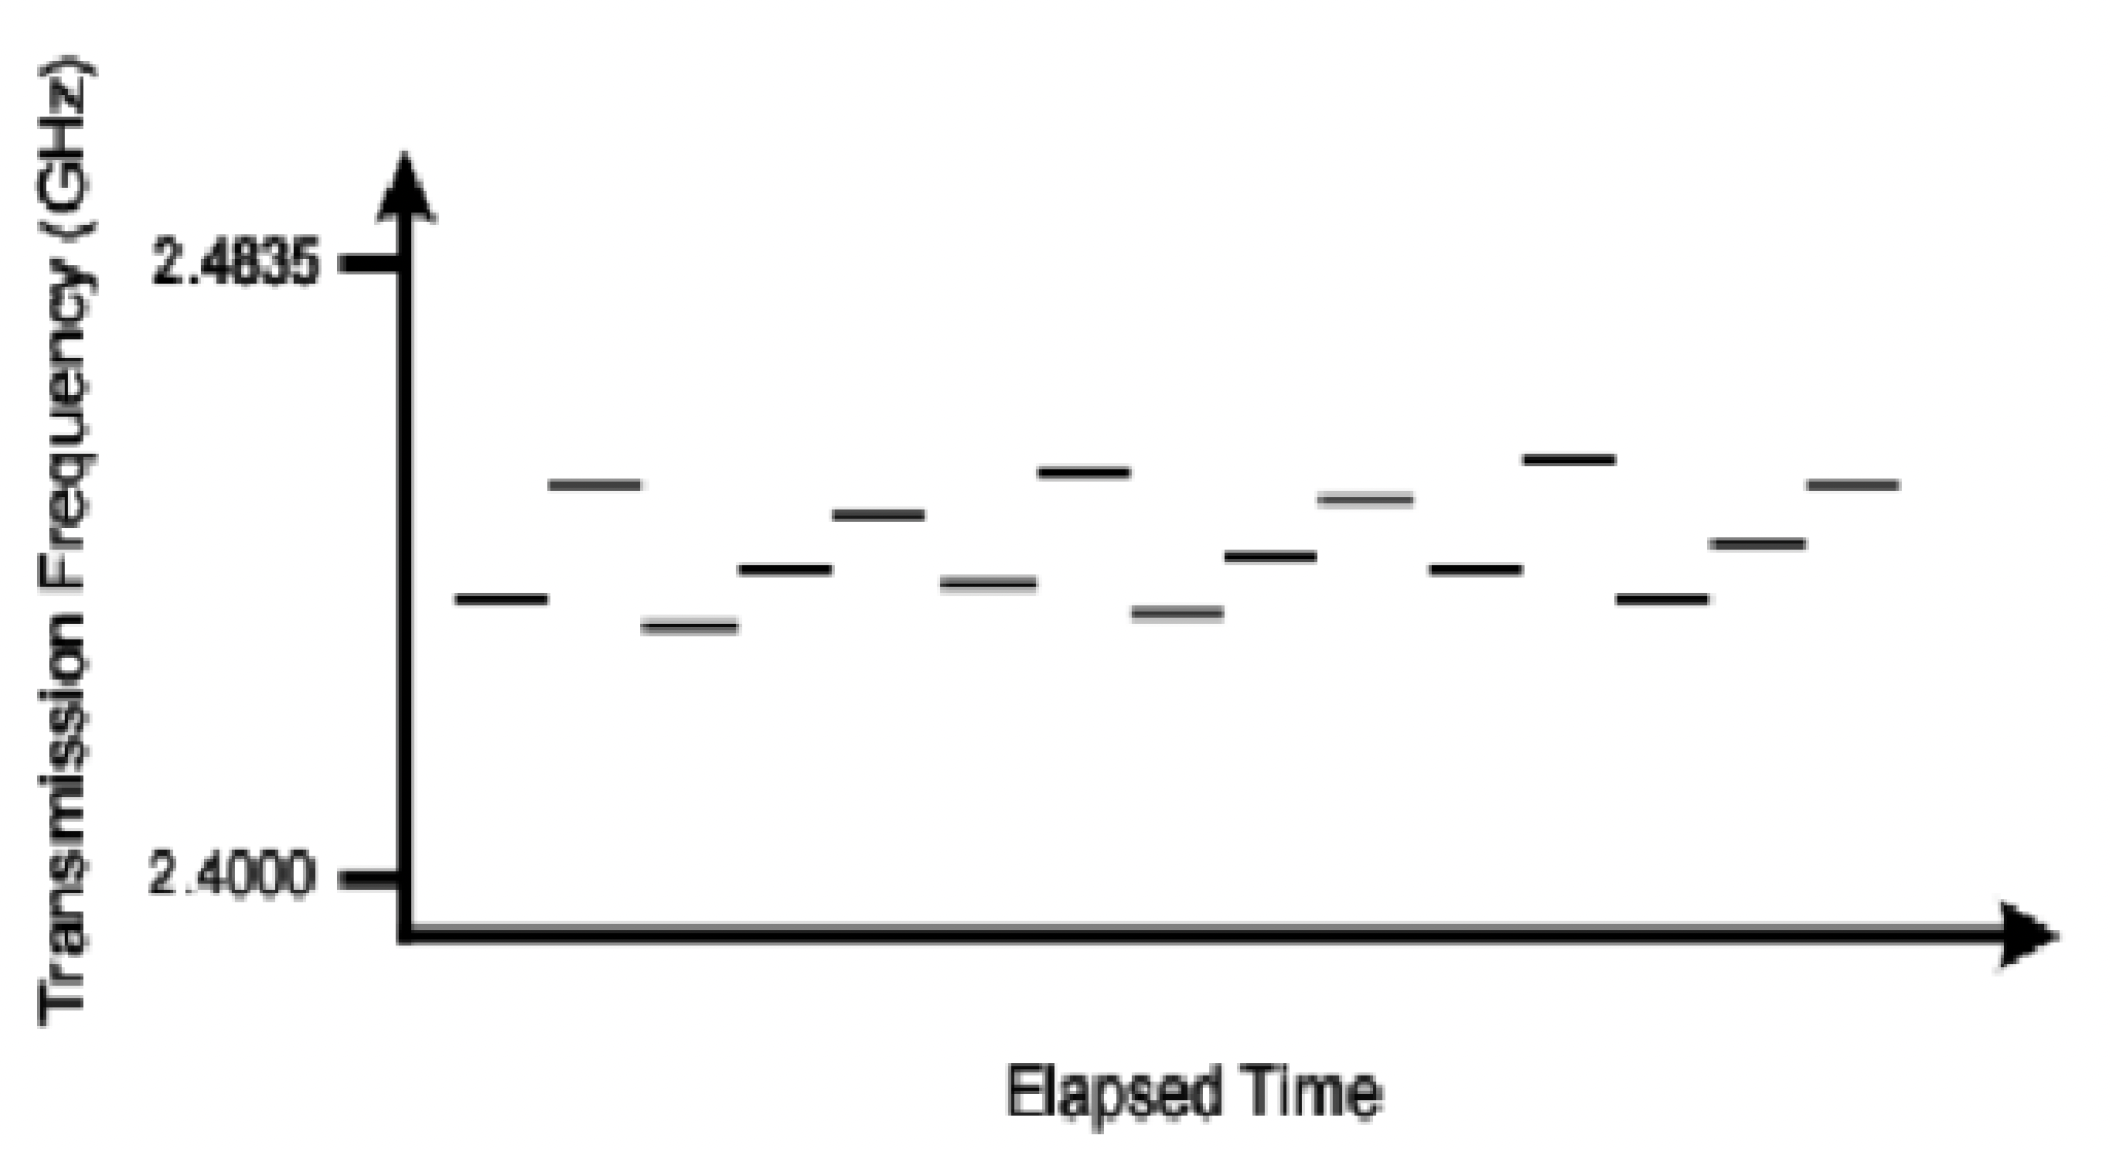
\includegraphics[width=.8\linewidth]{res/FHSS.png}
    \caption{}
\end{figure}

\subsection{Eavesdropping}
Anche utilizzando FHSS non verrà garantita la sicurezza del segnale, infatti eavesdropping e sniffing sono perpetrabili molto facilmente sulla trasmissione radio, sapendo il seed del PRNG che genera la sequenza di portanti potremo risalire alla sequenza stessa, basterà conoscere la modulazione e il protocollo utilizzato per effettuare l'attacco.
Esistono anche attacchi praticabili senza conoscere ne la modulazione ne il protocollo, questo prende io nome di \textbf{Reply Attack}. Sarà sufficiente catturare una porzione di segnali (spettro) e ritrasmetterle così come catturate.
Questo attacco non è protetto da meccanismi di integrità e confidenzialità, infatti è possibile integrare il messaggio seppur cifrato con altre informazioni ed esser considerato valido lo stesso.

Questo meccanismo di attacco viene utilizzato spesso dai cancelli automatici, catturato il treno di impulsi OOK sulla giusta portante sarà possibile reinviare il messaggio al cancello automatico per farlo aprire. Questa metodologia non prevede la comprensione del contenuto del messaggio inviato.

\subsection{Rolling Code}
Le automobili e i cancelli automatici più sicuri implementano un sistema di \textbf{Rolling Code};
\begin{itemize}
    \item il trasmettitore seleziona un codice basandosi su un PRNG e lo invia;
    \item il trasmettitore seleziona il codice successivo, basandosi sul PRNG;
    \item il ricevitore controlla che il codice ricevuto sia consistente con il suo PRNG, nel caso lo sia effettua l'operazione e fa avanzare il PRNG.
\end{itemize}
Un problema però del Rolling Code si presenta nel momento in cui il codice viene trasmesso e non ricevuto, questo porta a un disallineamento del PRNG e conseguentemente la non effettuazione del comando. Questa cosa si può risolvere facendo controllare al ricevitore non più un PRNG singolo ma una finestra nella quale il segnale sia valido, facendo poi avanzare la finestra di conseguenza. Questa cosa non risolve comunque l'attacco Reply ma lo rallenta rendendolo meno efficiente, obbligando l'attaccante a dover catturare più codici dal trasmettitore.

\subsection{Challenge and Response}
Il problema di questi metodi è la mancanza di un canale di ritorno. Infatti questi cancelli o macchine non dialogano con il trasmettitore ma si limitano a ricevere i comandi e ad eseguirli.
Tramite dei transceiver è possibile effettuare quello che si chiama \textbf{Challenge and Response}, presente anche in vari protocolli applicativi dunziona nel seguente modo:
\begin{itemize}
    \item L’autenticando (trasmettitore nei casi precedenti) richiede di accedere al sistema tramite un messaggio.
    \item L’autenticatore (cancello o macchina) genera un numero random (nonce) e lo invia all’autenticando.
    \item L’autenticando cifra il nonce inviato e reinvia il valore cifrato all’autenticatore.
    \item L’autenticatore decifra il valore cifrato e valida o meno l’autenticazione.
\end{itemize}
\begin{figure}[h!]
    \centering
    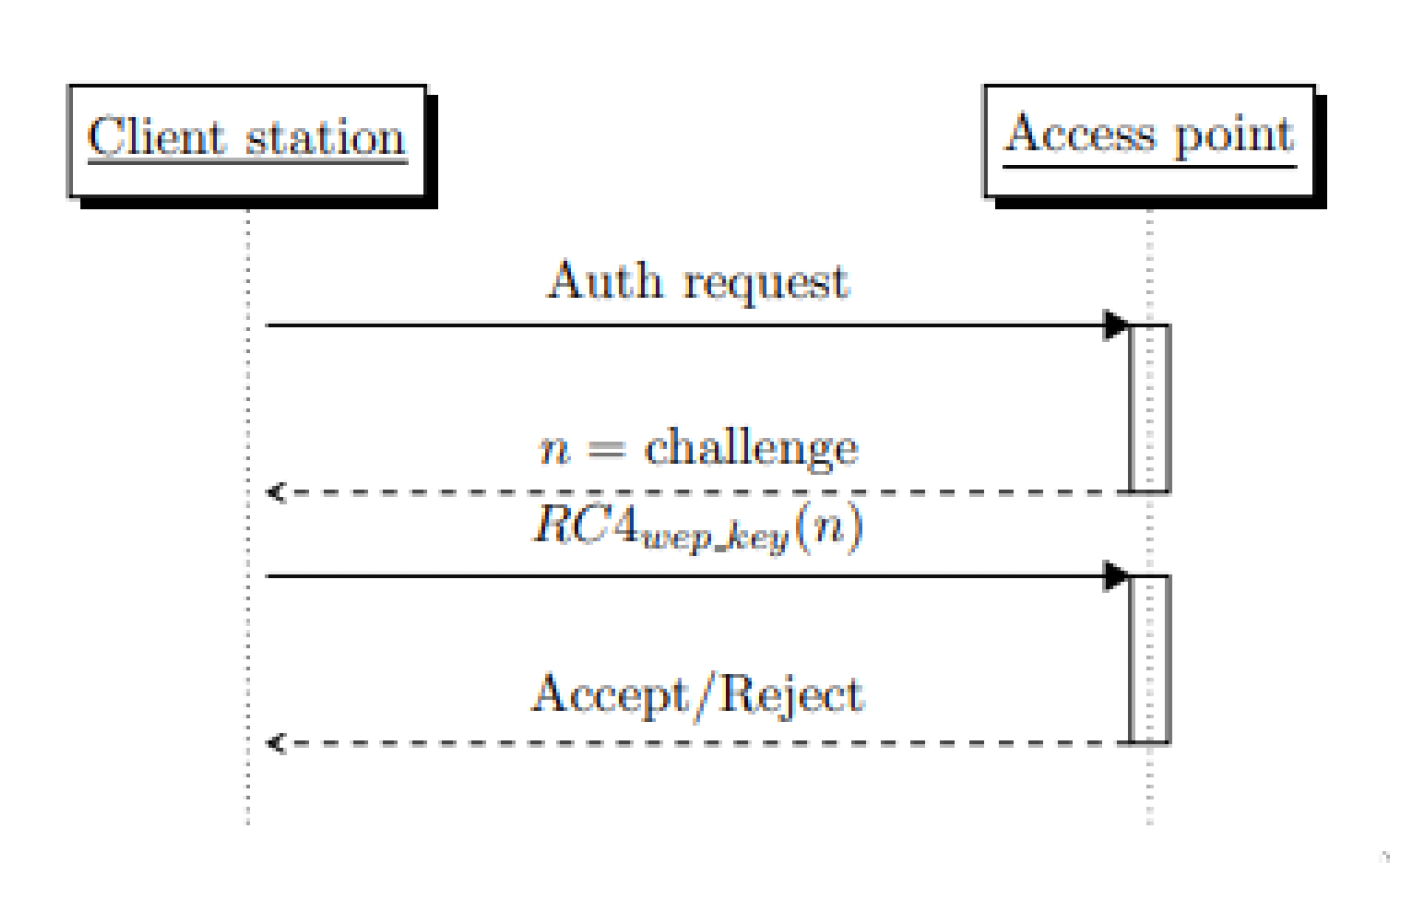
\includegraphics[width=.8\linewidth]{res/challenge_and_response.png}
    \caption{}
\end{figure}

\subsection{Cifratura}
Ovviamente la cifratura può essere applicata, oltre che ai meccanismi di autenticazione, anche per mantenere la confidenzialità e l'integrità dei dati in transito. Generalmente nelle radiotrasmissioni questa viene implementata tramite cifrari a blocchi (e.g. AES) o a flusso (e.g. Kasumi per il 4G).

\subsection{RFID}
Un altro sistema di autenticazione radio è l'RFID (Radio Frequency Identification) normalemente utilizzato per autenticare tramite bdage (e.g. Unibo), telefono o portachiavi.
Ad esempio i badge Unibo utilizzano una tecnologia chiamata EM410X, questa prevede un ID interno univoco e non sovrascrivibile assegnato dal database Unibo. In questo modo i portali in cui si richiede l'autenticazione effettueranno una ricerca nel database per controllare se l'account è effettivamente autorizzato ad accedere a un determinato varco.


\subsubsection{Cloning}
\textbf{I badge EM410X vengono venduti senza la possibilità di modificare l'ID associato, come si può aggirare questa protezione?}

Per aggirare questa protezione vi sono due metodi. Comprare un badge libero, oppure se la prima opzione non è percorribile, in assenza di meccanismi crittografici è sempre possibile spacciarsi per un badge con un transceiver RFID.

\section{IEEE 802.11 (Wi-Fi)}

\subsection{Introduzione}
Una delle comunicazioni radio più influenti nel mondo è senza ombra di dubbio lo standard \textbf{IEEE 802.11}, comunemente chiamato Wi-Fi.
Standard pensato per creare reti locali interoperabili con reti \textbf{Ethernet}.

\subsection{Layer Fisico}
Lo standard è diviso in altri sotto standard, e.g. IEEE 802.11g per le reti 2.4GHz o
IEEE 802.11ac per le reti operanti nella banda dei 5GHz, a seconda dello standard di afferenza il layer fisico alla base e la  modulazione può avere variazioni (per accesso al canale principalmente).
A livello fisico non vengono poste protezioni normalmente.
Essendo lo standard Wi-Fi basato anch'esso sulle onde radio, le onde propagate sono anch'esse sensibili a collisioni, per questo motivo avremo bisogno di un protocollo di accesso al canale tra i dispositivi in modo da risolvere eventuali collisioni.

Inoltre non è sempre possibile vedere tutti i nodi, il punto d'accesso normalmente ha visibilità in tutta la rete (se singolo), al contrario i singoli nodi no. Questo problema prende il nome di \textbf{Terminale Nascosto}.

\subsection{IFS (inter frame space)}

Il problema delle collisioni può essere mitigato accorgendosi della sua presenza e aspettando un tempo random prima di ritrasmettere il messaggio. Il protocollo prevede quindi degli "spazi" di silenzio che dovranno essere rispettati per evitare le collisioni. La gestione di questi spazi è particolarmente complessa con diverse classificazioni (e.g. spazi che solo l'access point dovrà attendere, spazi dedicati ai client ecc.) questi spazi prendono il nome di \textbf{}IFS (inter frame space).
\begin{figure}[h!]
    \centering
    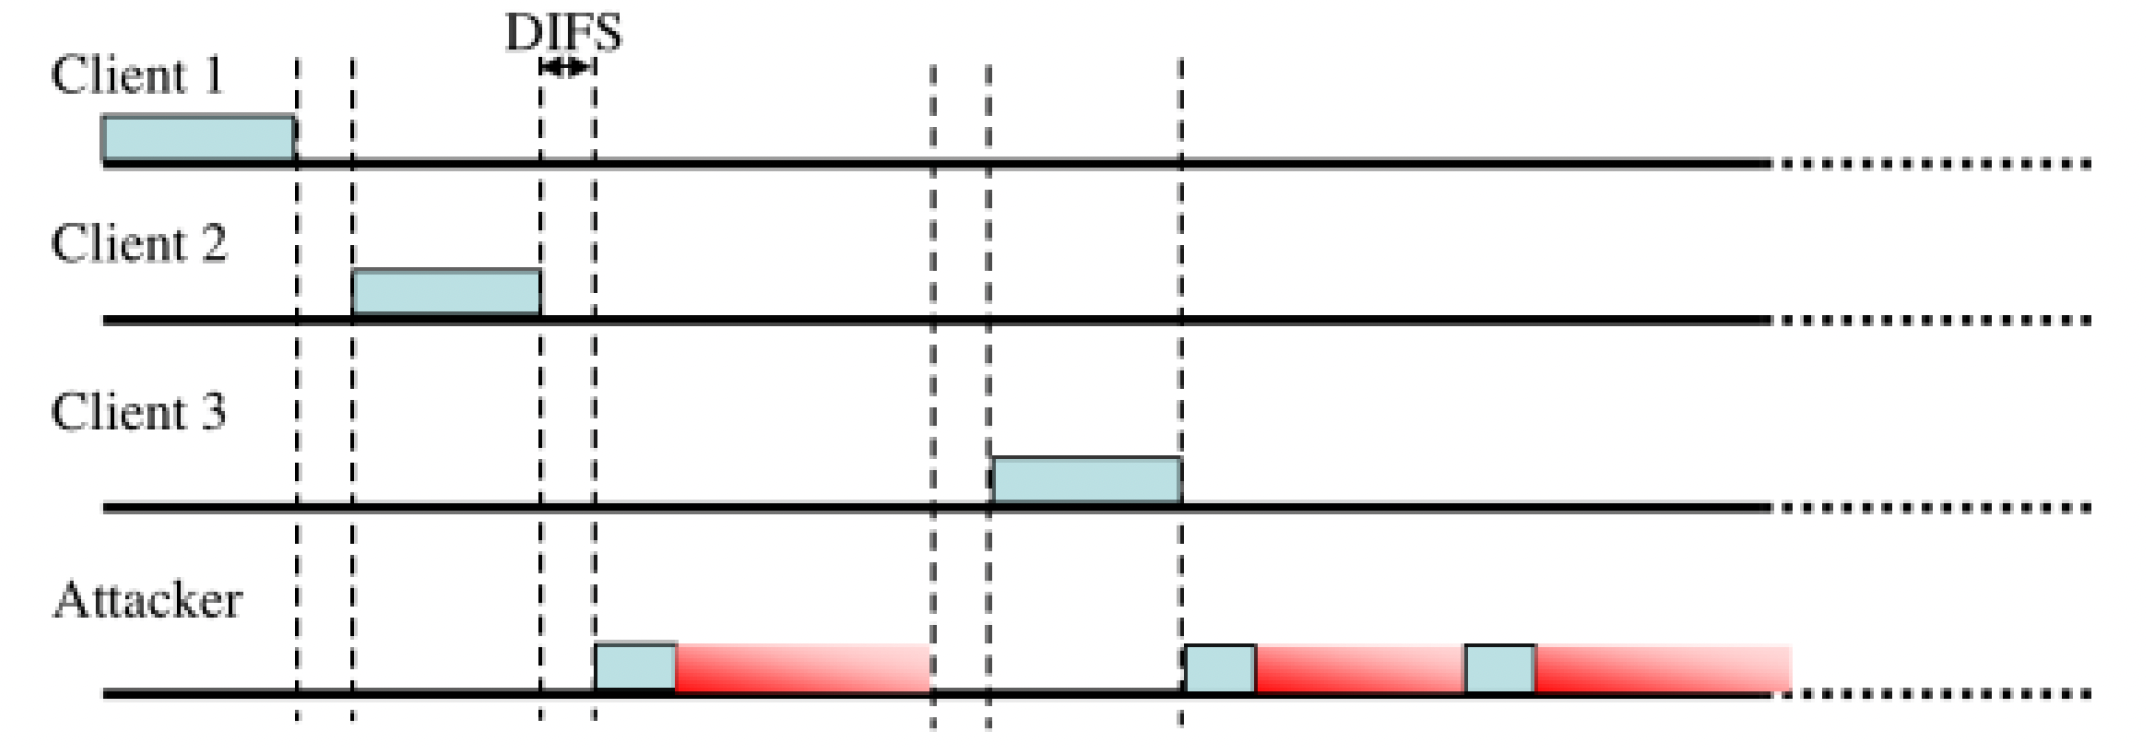
\includegraphics[width=.8\linewidth]{res/IFS.png}
    \caption{}
\end{figure}

\subsection{Denial of Service}
\textbf{Domanda:} Cosa succede se qualcuno non rispetta lo spazio di silenzio successivo a una collisione e non aspetta nessun IFS?

Perla sempre e solo lui.

\textbf{Domanda:} Cosa succede se due terminali non rispettano lo spazio di silenzio successivo a una
collisione e non aspettano nessun IFS?

Nessuno può più parlare!

\subsection{Sicurezza delle reti}

Un primo meccanismo di sicurezza, se così si può parlare, è nascondere il nome della rete, ciò obbliga gli hosts che si vogliono connettere di sapere a priori il nome della rete. Questa meccanismo non è comunque considerabile sicuro (security by obscurity).
Al livello 2, i terminali IEEE 802.11 utilizzano degli indirizzi Mac, esattamente come le
schede di rete Ethernet.
Un altro meccanismo di sicurezza implementabile è mediante l'utilizzo degli indirizzi mac, abilitando l'accesso alla rete solo a ad alcuni dispositivi, ciò comporta però il vincolo della rete solo a quei determinati dispositivi. Il problema di questo approccio, sempre security by obscurity, è che anche se la rete avrà un accesso limitato solo da parte di quei dispositivi, l'indirizzo mac è inviato in chiaro nel pacchetto, facilmente reperibile analizzando il traffico. Sarà quindi possibile effettuare facilmente uno “spoofing” sulla rete successivamente a una fase di sniffing per scoprire l'indirizzo mac di un host e utilizzarlo per connettersi.

\begin{lstlisting}[language=bash]
    command:
    macchanger -m 11.22.33.44.55.66 virbr0

    output: 
    Current MAC: 52:54:00:b7:9a:84 (unknow)
    Permanent MAC: 00:00:00:00:00:00 (XEROX CORPORATION)
\end{lstlisting}

L' autenticazione della rete e la confidenzialità per sistemi di questo tipo sono fondamentali, in quanto per fare eavesdropping non è richiesto il man in the middle.
In una rete aperta queste informazioni viaggiano tutte in chiaro rendendo possibile la lettura da chiunque, per questo motivo si mettono in atto sistemi di crittografici atti a proteggere le reti (cifrari).
Nonostante questi meccanismi di cifratura e accesso alla rete, lo standar prevede che determinati messaggi siano inviati in chiaro, senza nessun meccanismo di confidenzialità o anti replay (e.g. lo standar prevede che esista un messaggio di "disassociazione" a una rete, con questo messaggio
è possibile far sì che un terminale tolga l’associazione con un determinato access point).

\begin{figure}[h!]
    \centering
    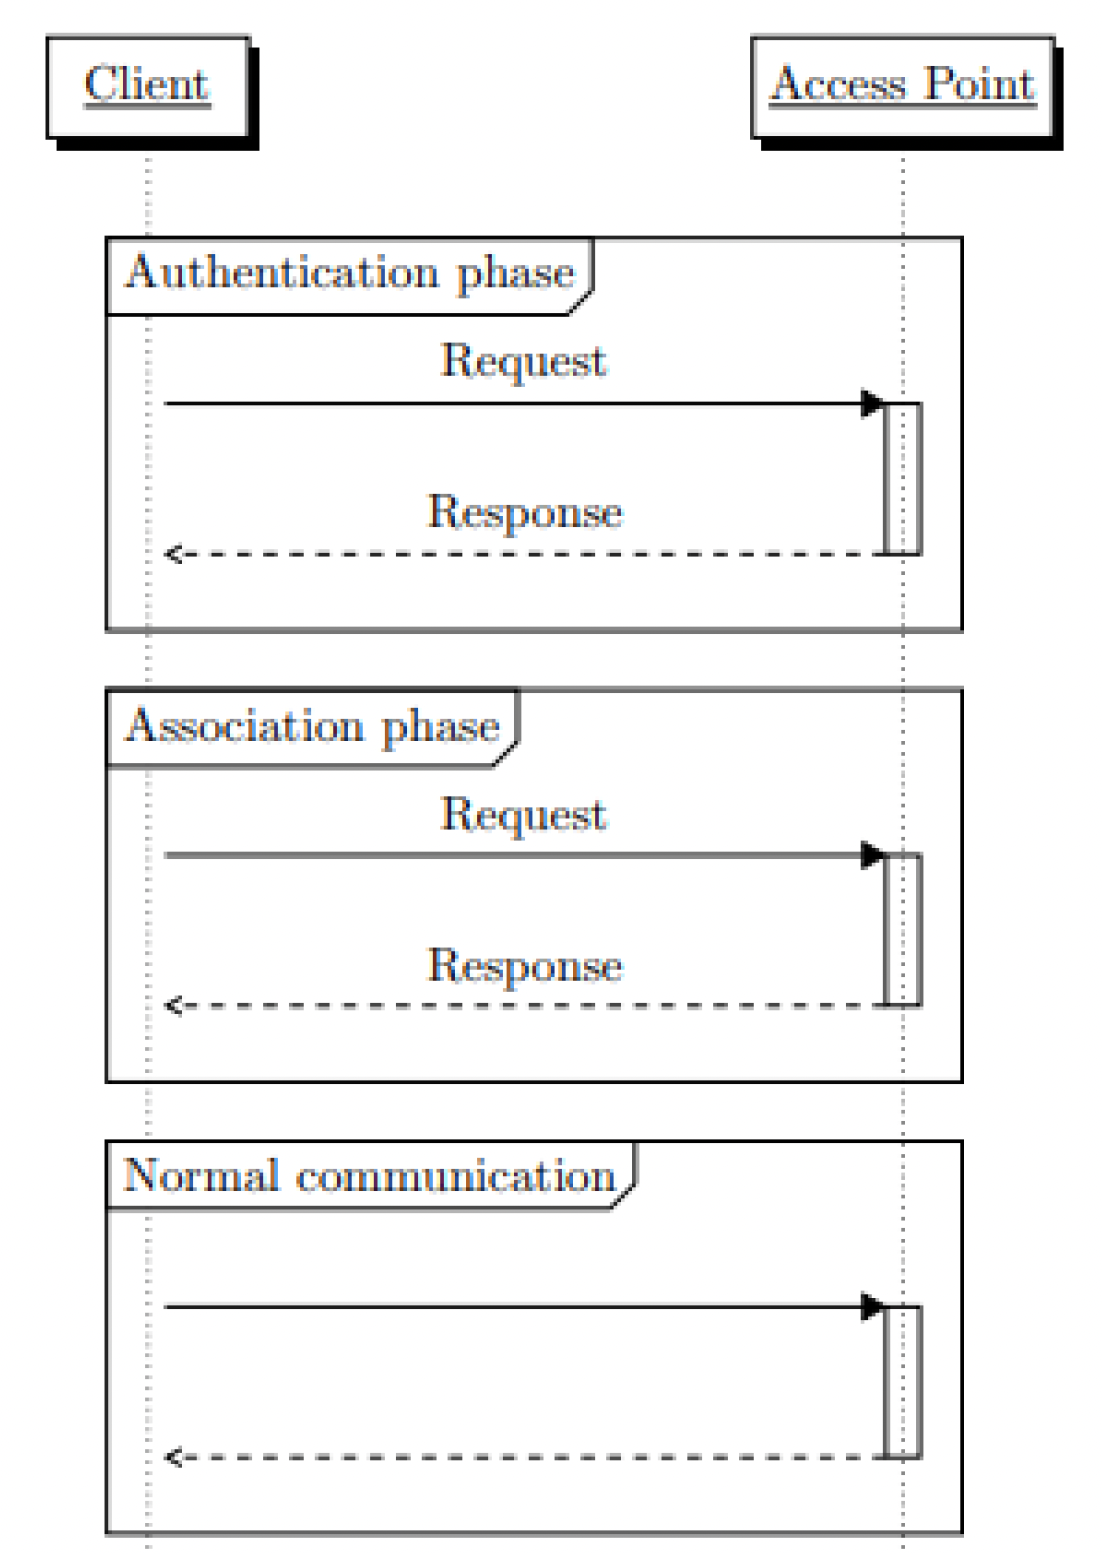
\includegraphics[width=.4\linewidth]{res/IEEE80211.png}
    \caption{}
\end{figure}

\subsection{WEP (Wired Equivalent Privacy)}
La prima forma di sicurezza pensata per le reti Wi-Fi è stata la \textbf{WEP (Wired Equivalent Privacy)}, ritenuto ormai non più sicuro, questo protocollo presenta due modalità:
\begin{itemize}
    \item Shared key;
    \item Open System.
\end{itemize}

Nella prima modalità, \textbf{Shared Key}, la possessione della chiave da parte dei client viene dimostrata attraverso un sistema di challenge and response, questa modalià è ormai considerata danno in quanto facilmente attaccabile attraverso attacchi di known plaintext (KPA) ricavando facilmente la chiave da tutte le autenticazioni.

\begin{figure}[h!]
    \centering
    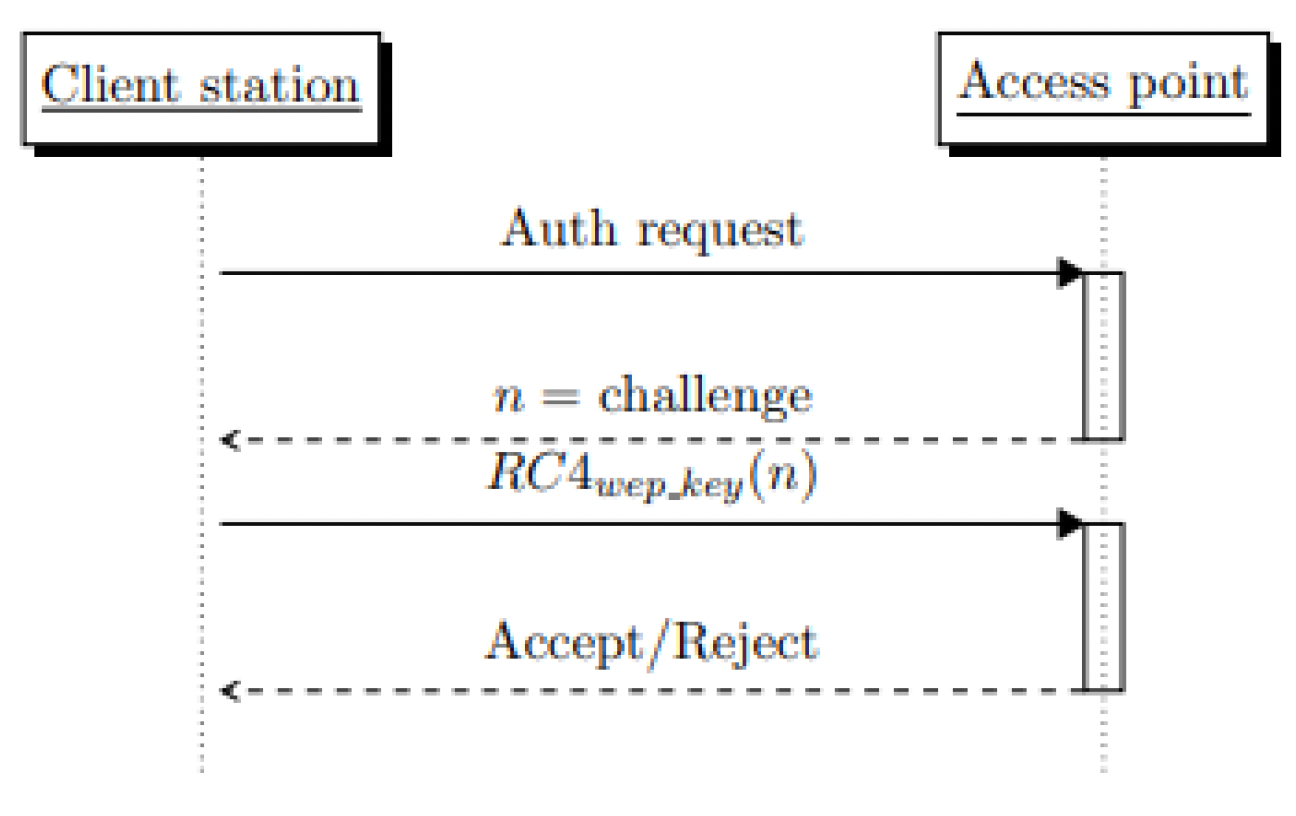
\includegraphics[width=.6\linewidth]{res/WEP_SharedKey.png}
    \caption{}
\end{figure}
\clearpage

Nella seconda modalità, \textbf{Open System}, il richiedente è già a conoscenza del segreto comune, ovvero la chiave condivisa, altrimenti non sarebbe in grado di decifrare i pacchetti cifrati
provenienti dall’access point.

\begin{figure}[h!]
    \centering
    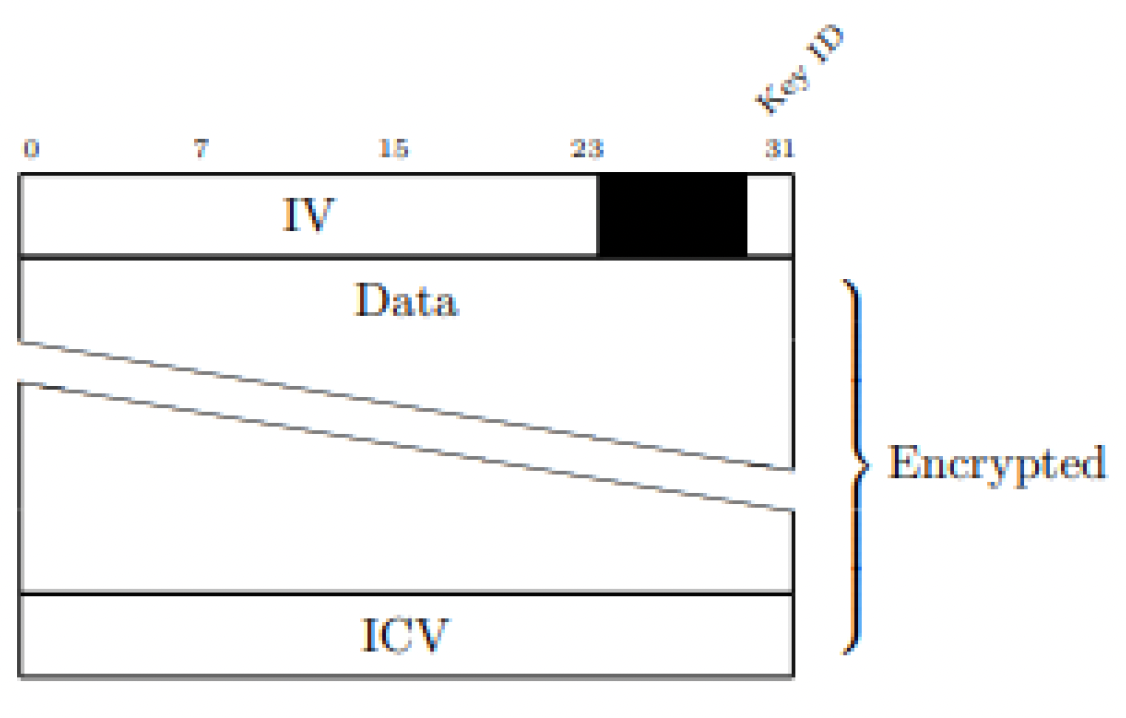
\includegraphics[width=.6\linewidth]{res/WEP_OpenSystem.png}
    \caption{}
\end{figure}

Mediante l'utilizzo di RC4, un algortimo di cifratura a flusso a chiave simmetrica. La Chiave WEP (da 40 o 104 bit) viene inizialmente concatenata con un vettore di inizializzazione (IV) a 24 bit in questo modo viene formata una stringa di 64 o 128 bit (40+24 o 104+24) che viene fornita in ingresso all’algoritmo RC4 per andare a creare la chiave di cifratura dei dati.

$
    m = m_0||m_1||m_2||...||m_n\\
    RC4_seed(IV||k)\\
    c_0 = RC4() \oplus m_0\\
    ...\\
    c_i = RC4() \oplus m_i\\
    ...\\
    c_n = RC4() \oplus m_n
$

Dopo 30000 pacchetti trasmessi dalla rete le probabilità di collisione sono praticamente impossibili da evitare.

$collisionP \approx 1 - e^\frac{-30000^2}{2*(2^{24})} = 0,99999999999774...$

Sapendo questo possiamo arrivare alla conclusione che catturando abbastanza pacchetti con lo steso IV si potranno fare attacchi statistici, inoltre catturando pacchetti con un IV noto sarà possibile far ricircolare pacchetti vecchi per aumentare il traffico della rete.

\subsection{WPA (Wi-Fi Protected Access)}
Per ovviare ai precedenti problemi di WEP si è sviluppato un nuovo protocollo più sicuro chiamato \textbf{WPA (Wi-Fi Protected Access)}, questo standard attualmente alla versione 3, pone diversi modi di utilizzo per il canale:
\begin{itemize}
    \item PSK, per reti domestica, chiave segreta su ogni dispositivo;
    \item Enterprise, per reti con molti utenti (e.g. ALMAWIFI);
    \item WPS, sistema di autenticazione facilitato;
\end{itemize}
che sfruttano diversi metodi di cifratura in base al caso:
\begin{itemize}
    \item TKIP, compatibile WEP, deprecato;
    \item CCMP, basato su AES (attuale standard).
\end{itemize}

\subsubsection{WPA-PSK TKIP}
Il primo metodo di autenticazione \textbf{WPA-PSK TKIP} è stato concepito per essere retrocompatibile con WEP, basandosi anch'esso su RC4 e con una gestione delle chiavi un pò più sicura, ciò ha portato a fargli ereditare gli stessi problemi di WEP. Ormai reso deprecato.

\subsubsection{WPA-PSK CCMP}
Al contrario del metodo precedente \textbf{WPA-PSK CCMP} utilizza un cifrario forte (AES) e una gestione delle chiavi molto più complessa, portandolo a risultare uno dei metodi più resistenti di WPA in questo momento

Seppur più sicuro tutte le reti PSK soffrono degli stessi problemi, cioè vulnerabilità a livello di autenticazione non di crittografia, ad esempio si potranno perpetrare comunque attacchi di tipo bruteforce o dizionario analogamente alle password.

\subsubsection{WPS}
Per rendere più semplice l'autenticazione ad una rete si è studiato un metodo per l'autenticazione ad una rete senza bisogno della password, abilitando diverse tipologie di accesso come mediante un pin o un pulsante fisico sul dispositivo di rete.

Un sistema utilizzante WPS potrà facilmente essere attaccato, mediante un rougue access point posizionato in un punto strategico, se utilizzante il metodo di accesso con pulsante fisico. Mentre se utilizzante l'accesso tramite PIN le cose si fanno ancora più pericolose in quanto essendo implementato attraverso 7 cifre, tramite un attacco bruteforce basteranno 10000000 tentativi per trovare la password. Per qualche scelta implementativa però si è deciso che le ultime 3 cifre del PIN vengano controllate solo se le prime 4 sono corrette abbassando così a 11000 tentativi (10000+1000) la ricerca, circa 20 ore.
Inoltre, l'implementazione di WPS su molti dispositivi embedded utilizzava un PRNG (nonce) predicibile, abbassando il tempo di bruteforce a pochi minuti catturando e analizzando la comunicazione.
Questi tipi di attacchi prendono il nome di \textbf{Pixiedust}.

\subsubsection{WPA-Enterprise}
Al contrario delle reti normali le reti enterprise per garantire il login prevedono un server chiamato Radius che mantiene il login degli utenti. Il primo passaggio della rete non è cifrato con nessuna chiave, ma funziona mediante un meccanismo di certificati, ciò crea la possibilità di sfruttare un rougue access point.
Normalmente la connessione viene effettuata tramite un meccanismo di challenge and response, rendendo possibile quindi per il rouge access point effettuare un crack della password bruteforce o a dizionario. Come per WPA-PSK esiste un metodo semplificato anche per l'accesso a una rete enterprise, questo prende il nome di \textbf{GTC (Generic Token Card)} e può essere richiesto come preferenziale per l'accesso. Di norma già abilitato sui dispositivi mobili, il protocollo disabilita la procedura di challenge and response inviando la password \textbf{in chiaro}.

\subsubsection{Krak}
Così come per WEP, fino a WPA2, era possibile un attacco di replay. Nella fase di autenticazione della rete viene utilizzato un nonce che può essere riutilizzato identico per velocizzare le successive connessioni. Questo porta a una falla di sicurezza in quanto si potranno reinstallare chiavi vecchie in modo da poter analizzare facilmente la comunicazione e risalire alla chiave di cifratura. Grazie a questo attacco lo standard è stato ulteriormente migliorato dando vita a WPA3.